%%
%% copyright quintard julien
%% 
%% kaneton
%% 
%% k2-subject.tex
%% 
%% path          /root/data/research/projects/svn/kaneton/projects/k2
%% 
%% made by mycure
%%         quintard julien   [quinta_j@epita.fr]
%% 
%% started on    Mon Feb 21 16:02:16 2005   mycure
%% last update   Sat Feb 26 10:49:20 2005   mycure
%%

\documentclass[10pt,a4wide]{article}
\usepackage[english]{babel}
\usepackage{a4wide}
\usepackage{graphicx}
\usepackage{graphics}
\usepackage{fancyheadings}
\pagestyle{fancy}

\bibliographystyle{plain}

\lhead{{\scriptsize kaneton project}}
\rhead{k2 subject}
\rfoot{\scriptsize EPITA System Lab}

\title{kaneton2}

\author{Julien Quintard - \small{quinta\_j@epita.fr} \\
        Jean-Pascal Billaud - \small{billau\_j@epita.fr} \\ \\
	\small{last updated by} \\
	Julien Quintard - \small{quinta\_j@epita.fr}}

\date{\today}

\begin{document}
\maketitle

\section{Informations}

\begin{tabular}{p{7cm}l}

Date de rendu: & Lundi 14 Mars 2005 \`a 23h42 \\
Dur\'ee du projet: & 2 semaines \\
Nom du fichier de rendu: & k2.tar.gz \\
Responsable du projet: & Julien Quintard - \small{quinta\_j@epita.fr} \\
                       & Jean-Pascal Billaud - \small{billau\_j@epita.fr} \\
Newsgroups d\'edi\'es: & epita.kaneton, epita.adm.sr \\
Langages: & asm, C \\
Architectures: & Intel 32-bit \\
Nombre de personnes par groupes: & 3 \`a 5

\end{tabular}

\section{Introduction}

\paragraph{}

Le but de ce projet est de mettre en place un certain nombre de gestionnaires.

\paragraph{}

Le but du projet pr\'ec\'edent \'etait de mettre en place un environnement
propice \`a l'ex\'ecution du kernel. Au lancement du kernel, celui-ci
sait qu'il est mapp\'e en m\'emoire haute, qu'il dispose de la segmentation
et de la pagination et qu'il peut acc\'eder aux structures de donn\'ees.

\paragraph{}

A pr\'esent le kernel doit \^etre capable de traiter les interruptions
mat\'erielles, les exceptions et les interruptions logicielles. Ainsi,
vous devrez d\'evelopper une API permettant d'int\'eragir avec les
p\'eriph\'eriques.

\paragraph{}

De plus, un gestionnaire de m\'emoire physique sera indispensable pour allouer
et lib\'erer de la m\'emoire physique.

\section{Travail Demand\'e}

\paragraph{}

Le projet consiste en la mise en place de plusieurs gestionnaires. Pour chacun
d'entre eux nous vous demandons de pr\'evoir une partie ind\'ependante du
processeur ainsi qu'une partie d\'ependante mais cela sera expliqu\'e
dans la section Portabilit\'e.

\paragraph{}

Voici les \'etapes \`a respecter:

\begin{enumerate}
\item gestionnaire d'espaces d'adressage.
\item gestionnaire de segmentation.
\item gestionnaire de m\'emoire physique.
\item gestionnaire d'interruptions et d'exceptions.
\item gestion du PIC.
\item d\'eveloppement d'un driver clavier.
\item d\'eveloppement d'un driver timer.
\item D\'eveloppement d'un interpr\'eteur de d\'emonstration qui lit
      une commande au clavier et effectue une op\'eration.
\end{enumerate}

\section{Interfaces}

\paragraph{}

Nous vous rappellons que vous \^etes libres d'utiliser une autre
interface. Dans ce cas il vous sera demand\'e une documentation expliquant
vos choix tr\`es pr\'ecis\'ement. Sans celle-ci votre travail serait
consid\'er\'e comme inachev\'e et non concordant avec le sujet.

\paragraph{}

Les fonctions des interfaces retournent \textbf{0} si tout s'est
pass\'e correctement ou \textbf{-1} s'il s'est produit une erreur.
Il vous est autoris\'e d'\'etendre la gestion des erreurs en
renvoyant une valeur n\'egative s'il s'est produit une erreur,
cette valeur correspondant \`a un type d'erreur pr\'ecis. Cette norme
sera suivie pour tous les projets, de k0 \`a kn.

\subsection{Console}

Nous vous laissons le choix de l'interface de la gestion de la console.

\paragraph{}

Toutefois la console devra permettre:

\begin{itemize}
\item l'affichage d'un caract\`ere: \textbf{cons\_print\_char}().
\item l'affichage d'une chaine de caract\`eres: \textbf{cons\_print\_string}().
\item l'affichage d'un nombre avec une base donn\'ee:
      \textbf{cons\_print\_num}().
\item l'affichage d'une chaine de format via la fonction \textbf{printf}() qui
      devra se trouver bien entendu dans la libc.
\item le scrolling.
\item l'affichage du backspace, en d'autres termes l'effacement
      d'un caract\`ere.
\item l'effacement complet de la console.
\item la red\'efinition des attributs de la console \`a n'importe quel moment.
\item la gestion du curseur, celui-ci \'etant controll\'e via I/O ports.
\end{itemize}

\subsection{Espace d'adressage}

\paragraph{}

Vous devez fournir une interface destin\'ee \`a la gestion des
espaces d'adressage.

\paragraph{}

Cette partie du syst\`eme sera compl\'et\'ee dans les projets suivants,
principalement dans k3, qui se chargera de toute la partie virtuelle et dans
k4 pour finaliser le tout. \`A noter que les seules entit\'es \`a appliquer
des op\'erations sur les espaces d'adressage sont: le gestionnaire de m\'emoire
physique, le gestionnaire de m\'emoire virtuelle et bien entendu le
gestionnaire d'espaces d'adressage.

\paragraph{}

Un espace d'adressage est compos\'e d'une structure de donn\'ees destin\'ee
\`a contenir suffisamment d'informations pour d\'ecrire la m\'emoire
utilis\'ee par un processus, que cette m\'emoire soit physique, virtuelle,
mapp\'ee, non mapp\'ee etc..

\paragraph{}

\hspace{1.5cm}int \textbf{as\_init}(void);

\paragraph{}

Cette fonction initialise la gestion des espaces adressage.

\paragraph{}

\hspace{1.5cm}int \textbf{as\_rsv}(t\_asid \textbf{*asid});

\paragraph{}

Cette fonction r\'eserve un espace d'adressage, c'est-\`a-dire une structure
de donn\'ees d\'ecrivant un espace d'adressage. La fonction se contente
de r\'eserver et d'initialiser la structure de donn\'ees puis de retourner
son identifiant.

\paragraph{}

\hspace{1.5cm}int \textbf{as\_get}(t\_asid \textbf{asid},
                                   t\_as \textbf{*as});

\paragraph{}

Cette fonction retourne l'adresse de la structure d\'ecrivant l'espace
d'adressage \`a partir de son identifiant. Cette fonction peut \^etre
consid\'er\'ee comme priv\'ee dans le sens o\`u seules les fonctions
influant sur les espaces d'adressage devraient y faire appel:
\textbf{pm\_rsv}(), \textbf{vm\_rel}() etc..

\paragraph{}

Pour rappel, les gestionnaires d'espace d'adressage, de m\'emoire physique
et de m\'emoire virtuelle fonctionnent ensemble pour garder traces des
allocations de m\'emoire sur un espace d'adressage.

\paragraph{}

\hspace{1.5cm}int \textbf{as\_rel}(t\_asid \textbf{asid});

\paragraph{}

Cette fonction lib\`ere l'espace d'adressage sp\'ecifi\'e.

\paragraph{}

\hspace{1.5cm}int \textbf{as\_clear}(void);

\paragraph{}

Cette fonction d\'etruit tous les espaces d'adressage.

\subsection{Segments}

\paragraph{}

Nous vous demandons de d\'evelopper une interface pour la gestion des
segments. Comme nous l'avons vu en cours, le gestionnaire
de segmentation sur processeur IA-32 inclut la gestion des segments
m\'emoire ainsi que la gestion des contextes processeur TSS.

\paragraph{}

Cette partie sera consid\'er\'ee comme \'etant la partie ``machine
dependent'' de la gestion de la m\'emoire physique. De ce fait votre
gestionnaire de segments pourra tout \`a fait coller au processeur
Intel, et c'est d'ailleurs ce que nous allons tenter de faire.
De plus un syst\`eme ne disposant pas de notion de segments ne souffrira
pas de cette impl\'ementation puisqu'il lui suffira de faire comme bon
lui semble.

\paragraph{}

Le but ici est de proposer une interface pour pouvoir manipuler principalement
les segments m\'emoire car les contextes processeurs TSS ne seront pas
utilis\'es dans kaneton.

\paragraph{}

Voici donc l'interface que nous vous proposons concernant la
gestion des segments.

\paragraph{}

Notez bien que chaque op\'eration sur les segments doit \^etre
visible imm\'ediatement une fois l'op\'eration termin\'ee.

\paragraph{}

\hspace{1.5cm}int \textbf{seg\_init}(void);

\paragraph{}

Cette fonction initialise la gestion des segments.

\paragraph{}

\hspace{1.5cm}int \textbf{seg\_add}(t\_paddr \textbf{start},
                                    t\_paddr \textbf{size},
                                    t\_pl \textbf{pl},
                                    t\_segtype \textbf{type},
                                    t\_segid \textbf{*segid});

\paragraph{}

Cette fonction se contente d'ajouter un segment et de le mettre en
place en l'indiquant au processeur.

\paragraph{}

L'argument \textbf{pl} repr\'esente le ``Privilege Level'': PL\_KERNEL,
PL\_SERVICE, PL\_USER mais \'egalement PL\_EXEC, PL\_READ, PL\_WRITE
alors que \textbf{type} repr\'esente le type du segment: SEG\_TYPE\_MEM,
SEG\_TYPE\_TSS.

\paragraph{}

La fonction devra remplir le param\`etre \textbf{segid} avec l'identifiant
du segment.

\paragraph{}

\hspace{1.5cm}int \textbf{seg\_modify}(t\_segid \textbf{segid},
                                       t\_paddr \textbf{start},
                                       t\_paddr \textbf{size},
                                       t\_pl \textbf{pl},
                                       t\_segtype \textbf{type});

\paragraph{}

Cette fonction modifie le segment identifi\'e via le param\`etre
\textbf{segid}.

\paragraph{}

\hspace{1.5cm}int \textbf{seg\_remove}(t\_segid \textbf{segid});

\paragraph{}

Cette fonction efface un segment en le retirant de la liste des segments
utilis\'es.

\paragraph{}

\hspace{1.5cm}int \textbf{seg\_clear}(void);

\paragraph{}

Cette fonction d\'etruit tous les segments pr\'esents.

\paragraph{}

Il est \`a noter qu'\'etant donn\'e que le gestionnaire de segments
renvoie des identifiants, cela implique que ce gestionnaire est capable
de retrouver la structure de donn\'ees \`a partir de l'identifiant. Cet aspect
se retrouvera dans chaque gestionnaire utilisant des identifiants. \`A vous
donc de mettre en place un m\'ecanisme pour retrouver un objet \`a partir
de son identifiant.

\paragraph{}

Il est important de bien comprendre que l'utilisant d'identifiants pour cette
partie est absolument inutile puisque faisant partie de la partie ``machine
dependent''. N\'eanmoins celle-ci est pr\'esente pour que vous vous
familiarisiez avec ce type de gestionnaires.

\paragraph{}

\`A Noter que si vous trouvez que garder une correspondance identifiant:objet
est trop lourd il vous est toujours possible de renvoyer l'adresse de l'objet,
cette adresse repr\'esentant par la m\^eme occasion l'identifiant de l'objet.
Cette m\'ethode fonctionne mais est bien entendu beaucoup moins propre car
aucun contr\^ole ne peut \^etre fait sur un identifiant.

\subsection{M\'emoire physique}

\paragraph{}

Il vous est \'egalement demand\'e de fournir une interface pour
l'utilisation de la m\'emoire physique. Comme nous venons de le voir,
la partie ``machine dependent'' du gestionnaire de m\'emoire physique
sera principalement compos\'ee du gestionnaire de segments. Voyons d\'esormais
l'interface de la partie ``machine independent''.

\paragraph{}

Libre \`a vous d'utiliser l'algorithme que vous estimez le plus performant,
propre, facile \`a impl\'ementer: bitmap, bitmap \'evolu\'e, zones etc.. via
la structure de donn\'ees appropri\'ee: tableau, liste chain\'ee, arbre etc..

\paragraph{}

\hspace{1.5cm}int \textbf{pm\_init}(t\_paddr \textbf{start},
                                    t\_paddr \textbf{size});

\paragraph{}

Cette fonction se charge d'initialiser le gestionnaire de m\'emoire physique.

\paragraph{}

\hspace{1.5cm}int \textbf{pm\_rsv}(t\_asid \textbf{asid},
                                   t\_paddr \textbf{*addr},
                                   t\_paddr \textbf{npages},
                                   t\_pmflags \textbf{flags});

\paragraph{}

Cette fonction a pour but d'allouer un nombre donn\'e de pages contig\"ues
de m\'emoire physique.

\paragraph{}

L'argument \textbf{*addr} doit \^etre rempli par la fonction, indiquant
l'adresse de la zone allou\'ee. L'argument \textbf{flags} indique les options
d'allocation: PM\_FLAG\_ANY, PM\_FLAG\_DMA etc..

\paragraph{}

L'allocateur de m\'emoire physique peut utiliser l'asid et les
propri\'et\'es sur les zones pour fusionner celles-ci, all\'egeant
la structure de donn\'ees utilis\'ee pour la gestion de la m\'emoire.

\paragraph{}

Cette op\'eration devra \'egalement modifier la structure de donn\'ees
d\'ecrivant l'espace physique dans l'\textbf{as} sp\'ecifi\'e, cela
dans l'unique but de garder les structures coh\'erentes.

\paragraph{}


\hspace{1.5cm}int \textbf{pm\_attr}(t\_asid \textbf{asid},
                                    t\_paddr \textbf{addr},
                                    t\_paddr \textbf{npages},
                                    t\_pattr \textbf{attr});

\paragraph{}

Cette op\'eration permet de modifier les attributs d'une page physique.
Les attributs pourraient \^etre: PM\_ATTR\_SHARE pour marquer la zone
comme partag\'ee, PM\_ATTR\_COW pour le ``copy-on-write'' ou m\^eme
PM\_ATTR\_AGGREGATE pour marquer une zone comme \'etant un objet. Ce dernier
attribut force le gestionnaire de m\'emoire physique \`a consid\'erer
cette zone comme elle est et non \`a fusionner ou d\'ecouper celle-ci.

\paragraph{}

\`A noter que cette fonction est en option, pour plus d'informations voir
la section Bonus.

\paragraph{}

\hspace{1.5cm}int \textbf{pm\_rel}(t\_asid \textbf{asid},
                                   t\_paddr \textbf{addr},
                                   t\_paddr \textbf{npages});

\paragraph{}

Cette fonction se contente de lib\'erer un certain nombre
de pages de m\'emoire physique.

\paragraph{}

M\^eme chose pour cette fonction, il faudra \'egalement intervenir sur
l'\textbf{as} sp\'ecifi\'e.

\paragraph{}

\hspace{1.5cm}int \textbf{pm\_flush}(t\_asid \textbf{asid});

\paragraph{}

Cette fonction lib\`ere toute la m\'emoire physique que l'espace d'adressage
\textbf{asid} utilise.

\paragraph{}

M\^eme chose pour cette fonction, il faudra \'egalement intervenir sur
l'\textbf{as} sp\'ecifi\'e.

\paragraph{}

\hspace{1.5cm}int \textbf{pm\_clear}(void);

\paragraph{}

Cette fonction r\'einitialise la gestion de la m\'emoire physique en lib\'erant
toutes les pages de m\'emoires physiques r\'eserv\'ees.

\subsection{Interruptions/Exceptions}

\paragraph{}

La gestion des interruptions et des exceptions sur processeur Intel se fait
gr\^ace \`a une table nomm\'ee IDT.

\paragraph{}

Voici l'interface a utiliser pour la gestion des interruptions et exceptions
Intel.

\paragraph{}

Cette partie repr\'esente la partie totalement ``machine dependent'' de la
gestion des traps mais fera \'egalement partie de la partie
``machine dependent'' des messages. Pensez \`a organiser le code convenablement
pour \'eviter la duplication de code inutilement.

\paragraph{}

\hspace{1.5cm}int \textbf{int\_init}(void);

\paragraph{}

Cette fonction initialise la gestion des interruptions.

\paragraph{}

\hspace{1.5cm}int \textbf{int\_rsv}(u\_int8\_t \textbf{entry},
                                    t\_inttype \textbf{type},
                                    t\_segid \textbf{segid},
                                    t\_pl \textbf{pl},
                                    t\_vaddr \textbf{handler});

\paragraph{}

Cette fonction ajoute un handler sur le vecteur d'interruption \textbf{entry}.
Le param\`etre \textbf{type} repr\'esente le type de handler \`a g\'erer:
INT\_TYPE\_INT, INT\_TYPE\_TRAP, INT\_TYPE\_TASK ou INT\_TYPE\_CALL. L'argument
\textbf{segid} repr\'esente le segment contenant le handler et \textbf{pl}
repr\'esente les privil\`eges de l'interruption.

\paragraph{}

\`A savoir que nous utiliserons seulement le type INT\_TYPE\_INT, mais
ce point tr\`es pr\'ecis sera explicit\'e ult\'erieurement.

\paragraph{}

\hspace{1.5cm}int \textbf{int\_modify}(u\_int8\_t \textbf{entry},
                                       t\_inttype \textbf{type},
                                       t\_segid \textbf{segid},
                                       t\_pl \textbf{pl}, \\
\bigskip
\hspace{4.3cm}                         t\_vaddr \textbf{handler});

\paragraph{}

Cette fonction modifie une interruption d\'ej\`a enregistr\'ee.

\paragraph{}

\hspace{1.5cm}int \textbf{int\_rel}(u\_int8\_t \textbf{entry});

\paragraph{}

Cette fonction lib\`ere une entr\'ee de la table d'interruptions.

\paragraph{}

\hspace{1.5cm}int \textbf{int\_clear}(void);

\paragraph{}

Cette fonction r\'einitialise la gestion des interruptions.

\subsection{Clavier}

\paragraph{}

L'interface du driver clavier est laiss\'ee au choix du groupe pour certaines
raisons, la premi\`ere \'etant le fait que cette interface devra \'evoluer
avec le temps.

\paragraph{}

Inutile donc de s'acharner sur la mod\'elisation. N\'eanmoins nous vous
conseillons de faire un driver complet pour ne pas avoir de probl\`emes
plus tard.

\subsection{PIC}

\paragraph{}

Le PIC est encore une fois un \'el\'ement trop sp\'ecifique. Pour cette
raison la gestion du PIC sera incluse dans la partie ``machine dependent''.

\paragraph{}

\hspace{1.5cm}int \textbf{pic\_init}(void);

\paragraph{}

Cette fonction initialise la gestion du PIC.

\paragraph{}

\hspace{1.5cm}int \textbf{pic\_enable}(t\_eventid \textbf{eventid});

\paragraph{}

Cette fonction active l'interruption \textbf{eventid}.

\paragraph{}

\hspace{1.5cm}int \textbf{pic\_disable}(t\_eventid \textbf{eventid});

\paragraph{}

Cette fonction d\'esactive l'interruption \textbf{eventid}.

\paragraph{}

\hspace{1.5cm}int \textbf{pic\_clear}(void);

\paragraph{}

Cette fonction r\'einitialise la gestion du PIC.

\subsection{Timer}

\paragraph{}

L'interface du timer est laiss\'ee au choix du groupe.

\paragraph{}

Le but \'etant de g\'erer les interruptions timer et de retenir le nombre
de \textbf{ticks} \'ecoul\'es.

\section{Types}

\paragraph{}

Voici une explication plus compl\`ete des nouveaux types que
vous devrez utilis\'es.

\paragraph{}

Nous vous exposons ici un exemple de d\'efinition de ces types. Rien ne vous
oblige \`a les suivre.

\subsection{t\_paddr}

\paragraph{}

Ce type repr\'esente une adresse physique. Ce type sera d\'efini par la
partie ``machine dependent'' de kaneton pour des raisons \'evidentes de
portabilit\'e sur des architectures diff\'erentes style 64-bit par exemple.

\begin{verbatim}
typedef u_int32_t       t_paddr;
\end{verbatim}

\subsection{t\_vaddr}

\paragraph{}

Ce type repr\'esente une adresse virtuelle. M\^eme chose que pour
\textbf{t\_paddr}, ce type sera d\'efini pour la partie ``machine dependent''.

\begin{verbatim}
typedef u_int32_t       t_vaddr;
\end{verbatim}

\subsection{t\_asid}

\paragraph{}

Ce type identifie un espace d'adressage et n'est compos\'e que
d'un identifiant soit un nombre.

\begin{verbatim}
typedef u_int32_t       t_asid;
\end{verbatim}

\subsection{t\_as}

\paragraph{}

Ce type d\'ecrit un espace d'adressage et est compos\'e d'un identifiant et
de deux structures de donn\'ees, l'une d\'ecrivant l'espace physique utilis\'e
par cet espace d'adressage et l'autre d\'ecrivant l'espace virtuel utilis\'e
par ce m\^eme objet.

\begin{verbatim}
typedef struct          s_as
{
  t_asid                asid;
  [pas_data_structure]  pas;
  [vas_data_structure]  vas;
}                       t_as;
\end{verbatim}

\subsection{t\_pl}

\paragraph{}

Ce type repr\'esente un ensemble de privil\`eges. Attention le fait
d'utiliser le flag PL\_USER ne signifie pas du tout que le CPL sera
d\'efinit \`a \textbf{2}. Cela d\'efinit juste une valeur pour savoir
que cet objet aura les privil\`eges utilisateur, la partie d\'ependante
pourra donc choisir ais\'ement les valeurs \`a inscrire au niveau hardware.

\begin{verbatim}
#define PL_KERNEL       0x00
#define PL_SERVICE      0x01
#define PL_USER         0x02

#define PL_READ         0x04
#define PL_WRITE        0x08
#define PL_EXEC         0x10

typedef u_int16_t       t_pl;
\end{verbatim}

\subsection{t\_segtype}

\paragraph{}

Repr\'esente les types de segment disponible.

\paragraph{}

Cette partie fait totalement partie de la partie ``machine dependent''
\'etant donn\'e que la notion de segment n'est pas g\'en\'erique.

\begin{verbatim}
#define SEG_TYPE_MEM    0x00
#define SEG_TYPE_TSS    0x01

typedef u_int8_t        t_segtype;
\end{verbatim}

\subsection{t\_segid}

\paragraph{}

Ce type identifie un segment et n'est compos\'e que d'un identifiant soit
un nombre.

\paragraph{}

Cette partie fait encore totalement partie de la partie ``machine dependent''.

\begin{verbatim}
typedef u_int32_t       t_segid;
\end{verbatim}

\subsection{t\_pmflags}

\paragraph{}

Repr\'esente les diff\'erents flags qu'utilise la gestion de la m\'emoire
physique.

\begin{verbatim}
#define PM_FLAG_ANY     0x00
#define PM_FLAG_DMA     0x01

/*
 * ...
 */

typedef u_int16_t       t_pmflags;
\end{verbatim}

\subsection{t\_inttype}

\paragraph{}

Repr\'esente les diff\'erents types d'interruptions g\'er\'es par
l'architecture IA-32.

\paragraph{}

Cette partie fait totalement partie de la partie ``machine dependent''
\'etant donn\'e que la notion d'interruption n'est pas g\'en\'erique.

\begin{verbatim}
#define INT_TYPE_INT    0x00
#define INT_TYPE_TRAP   0x01
#define INT_TYPE_TASK   0x02
#define INT_TYPE_CALL   0x03

typedef u_int8_t        t_inttype;
\end{verbatim}

\subsection{t\_eventid}

\paragraph{}

Ce type repr\'esente un \'ev\`enement hardware. Inutile de s'\'etendre sur
le sujet, ces notions seront approfondies dans les sujets suivants.

\paragraph{}

Pour k2, un \'ev\`ement hardware est tout simplement caract\'eris\'e par
l'IRQ du p\'eriph\'erique. Gr\^ace \`a cela vous pourrez tester vos
drivers etc..

\begin{verbatim}
typedef u_int32_t       t_eventid;
\end{verbatim}

\newpage

\section{Visualisation}

\paragraph{}

Voici une visualisation de l'interaction entre la partie
``machine independent'' et la partie ``machine dependent'' suivi
d'une explication de chaque sous partie.

\paragraph{}

\begin{figure}[h]
\centerline{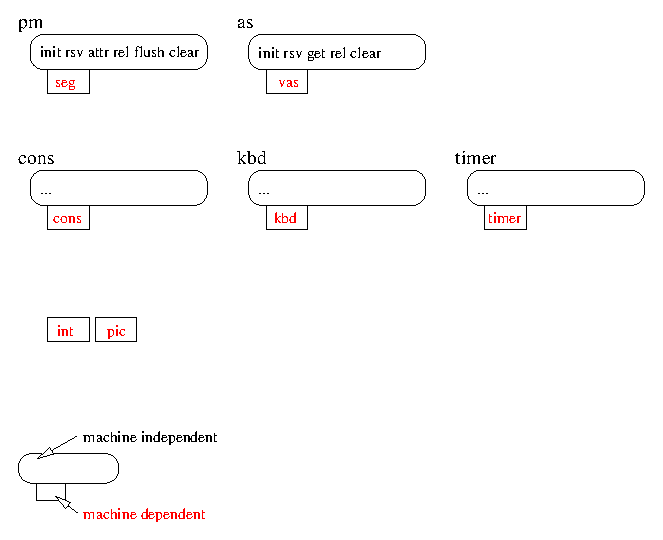
\includegraphics{figures/visualisation.eps}}
\end{figure}

\subsection{pm}

\paragraph{}

La partie ind\'ependante de l'architecture se contente de g\'erer les
structures de donn\'ees d\'ecrivant les espaces d'adressage physique,
c'est-\`a-dire un espace d'adressage physique par espace d'adressage
et un espace physique g\'en\'eral qui repr\'esente la m\'emoire
physique du syst\`eme.

\paragraph{}

La partie d\'ependante se contente de g\'erer les structures de donn\'ees
hardware en rapport avec la gestion de la m\'emoire physique.

\paragraph{}

Dans le cas de l'architecture IA-32, il vous suffira \`a l'initialisation de la
m\'emoire physique de cr\'eer tous les segments n\'ecessaires.

\subsection{as}

\paragraph{}

La partie ind\'ependante de l'architecture de la gestion des espaces
d'adressage se contente de g\'erer les structures de donn\'ees
g\'en\'eriques: la structure de donn\'ees d\'ecrivant l'espace physique
et celle d\'ecrivant l'espace virtuel.

\paragraph{}

Le seul but des fonctions de gestion de l'espace d'adressage est de
r\'eserver, de lib\'erer ou de retrouver un espace d'adressage.

\paragraph{}

Les structures internes aux espaces d'adressage ne sont modifi\'ees que
par le gestionnaire de m\'emoire physique et le gestionnaire de m\'emoire
virtuelle.

\paragraph{}

La partie d\'ependante se contentera de mettre en place les structures
hardware.

\paragraph{}

Sur l'architecture IA-32 par exemple, lors de la r\'eservation
d'un espace d'adressage, la partie d\'ependante devra r\'eserver une page
physique pour y stocker le \textbf{page directory} et l'initialiser. La
partie d\'ependante s'occupant de cette partie sur le sch\'ema se nomme
\textbf{vas}. Attention cette partie ne sera d\'evelopp\'ee que dans k3.
La partie \textbf{pas} ne devrait rien avoir \`a faire sur IA-32.

\subsection{int}

La gestion des interruptions est une partie totalement d\'ependante de
l'architecture. Celle ci devra donc \^etre construite pour pouvoir
coller ensuite avec les traps.

\subsection{pic}

La gestion du PIC est soumise est m\^eme contraintes que le gestionnaire
d'interruptions.

\section{Hi\'erarchie}

\paragraph{}

Comme vous pouvez le constater, il existe une hi\'erarchie.

\paragraph{}

La couche ``machine independent'' d\'el\`egue du travail via les interfaces
aux couches ``machine dependent''.

\paragraph{}

Cette hi\'erarchie ne doit jamais \^etre bris\'ee sans quoi le mod\`ele
deviendra incoh\'erent.

\section{Portabilit\'e}

\paragraph{}

La question qui subsiste est: Comment bien dissocier la partie ``machine
dependent'' de la partie ``machine independent''? Comment lancer, par
exemple, la fonction \textbf{seg\_init}() sur l'architecture IA-32 mais par sur
l'architecture Sparc?

\paragraph{}

Nous vous proposons ici une solution que vous pouvez choisir d'adopter ou non.

\begin{verbatim}

-- kernel/ia-32/pm.c

typedef struct  s_pm_dep
{
  int           (*pm_init)(t_paddr      start,
                           t_paddr      size);
  /*
   * pm_rsv, pm_attr, pm_rel, pm_clean
   *
   * ...
   */
}               t_pm_dep;

t_pm_dep        pm_dep =
{
  ia32_pm_init,
  ia32_pm_rsv,
  ia32_pm_rel,
  ia32_pm_clean,
};

int             ia32_pm_init(t_paddr    start,
                             t_paddr    size)
{
  seg_init();

  seg_add(...);
  seg_add(...);
  seg_add(...);
  seg_add(...);

  /*
   * ...
   */

  return (0);
}

-- kernel/pm.c

int             pm_init(t_paddr         start,
                        t_paddr         size)
{
  if (pm_dep.pm_init != NULL)
    pm_dep.pm_init(start, size);

  /*
   * ...
   */

  return (0);
}

/*
 * pm_rsv, pm_attr, pm_rel, pm_clean
 *
 * ...
 */
\end{verbatim}

\paragraph{}

L'utilisation de structure d\'ecrivant les fonctions d\'ependantes de
l'architecture \`a appeller permet aux architectures qui n'ont pas
besoin de fonctionnalit\'es d\'ependantes de l'architecture de ne
pas \^etre oblig\'ees de d\'efinir des fonctions vides. La seule d\'eclaration
requise \'etant la structure d\'efinissant les fonctions d\'ependantes
de l'architecture \`a appeller.

\paragraph{}

Encore une fois cette impl\'ementation est pratique car la partie
ind\'ependante ne se soucie de rien mis \`a part du fait qu'une structure
d\'ecrivant les fonctions d\'ependantes de l'architecture existe.

\paragraph{}

\`A vous de voir ce qu'il serait ing\'enieux de rajouter en param\`etre.
De plus il serait int\'eressant de rajouter un champ dans vos structures
de donn\'ees ind\'ependantes pour que les parties d\'ependantes puisse
stocker des informations.

\section{Bonus}

\paragraph{}

Voici les bonus de ce projet.

\subsection{Attributes}

Un ajout int\'eressant dans la gestion de la m\'emoire physique sera
de permettre le partage de pages physiques et plus particuli\`erement
la modification des attributs de pages physique.

\paragraph{}

Votre gestionnaire de m\'emoire physique devra donc garder une trace sur
le nombre de personnes utilisant une page ou une zone de pages physiques.

\paragraph{}

Lorsqu'une page partag\'ee par plusieurs espaces d'adressage est lib\'er\'ee
il faut d\'ecr\'ementer le nombre d'espaces d'adressage l'utilisant. Si ce
compteur tombe \`a zero alors la page peut \^etre lib\'er\'ee.

\paragraph{}

Une optimisation sera d'introduire un syst\`eme de protection pour que
seuls les espaces d'adressage autoris\'es puissent mapper cette page
partag\'ee.

\paragraph{}

De plus il vous sera demander de g\'erer les attributs COW et AGGREGATE.

\subsection{Tty}

Il pourrait \^etre int\'eressant de disposer de diff\'erents tty, c'est \`a
dire des couples console - clavier diff\'erent.

\paragraph{}

Il vous sera donc demand\'e de fournir un interface compl\`ete pour la
manipulation des tty.

\subsection{Clock}

La gestion de l'heure peut \^etre int\'eressant. Il vous sera donc
demand\'e de toujours avoir une date mise \`a jour.

\paragraph{}

Bien entendu il vous sera \'egalement demand\'e de fournir une commande
dans l'interpr\'eteur afin de mettre en valeur votre travail.

\subsection{Objects: ``Sharing sux''}

\paragraph{}

Pour les plus courageux nous vous proposons la mod\'elisation d'un nouveau
syst\`eme pour le partage de donn\'ees d'une mani\`ere plus propre que
le partage de pages.

\paragraph{}

Ce syst\`eme est bas\'e sur l'utilisation d'objets et est donc beaucoup
plus haut niveau que le partage de pages.

\paragraph{}

Nous vous demandons donc une mod\'elisation compl\`ete d'un tel syst\`eme
avec bien entendu une impl\'ementation. Le papier d\'ecrivant votre
syst\`eme devra comprendre les avantages et inconv\'enients d'un tel
syst\`eme.

\paragraph{}

Vous indiquerez \'egalement dans votre description si il est utile de
permettre aux processus, services etc.. d'allouer directement de la
m\'emoire physique avec un tel syst\`eme.

\paragraph{}

Ce bonus est destin\'e \`a vous faire r\'efl\'echir sur les syt\`emes
existants et sur ce qu'un syst\`eme \`a base d'objets peut permettre.

\paragraph{}

Attention nous utilisons ici le terme d'objet mais par forc\'ement au sens
complet: donn\'ees internes et m\'ethodes. C'est \`a vous d'imaginer un
syst\`eme en C qui apporte la propret\'e des objets avec si possible
un syst\`eme de contr\^ole sur les acc\`es aux objets.

\paragraph{}

Ce syst\`eme devra permettre le partage d'objets par plusieurs entit\'es
qui auront pr\'ealablement \'et\'e autoris\'ees par l'entit\'e ma\^itre de
l'objet.

\paragraph{}

Bien entendu, l'acc\`es aux objets utilisera forc\'ement une
exclusion mutuelle.

\end{document}
